%==============================================================================%
%  THE PROJECT GROUP LATEX TEMPLATE
%  Complex and Distributed IT-Systems
%  Technische Universiaet Berlin
%------------------------------------------------------------------------------%
%  FILE HISTORY: 
%    o 2005-12-21 HSL/TF: Initial version
%    o 2006-03-14 HSL   : Different headings for odd and even pages,
%                         simple setup mechanism (see @SETTINGS).
%    o 2009-06-09 DW:			Adapted to match TUB/CIT layout
%------------------------------------------------------------------------------%
%  QUICK START:
%  You need to perform few settings in order to use this LaTeX template.
%  Look for comments starting with @SETTINGS to locate the lines that
%  require modifications.  Basically, this is what needs to be done:
%    o Select the right encoding (for most users either applemac or latin1
%      will do).
%    o Enter your name in the definition of the command \pgauthor.
%    o Enter the title of the document in the definition of the command
%      \pgtitle.
%    o If you're using this template for your seminar paper, make sure that
%      \cfoot{} is not commented!  This disables all page numbers.
%    o Decide whether you want a table of contents and/or a list of figures.
%      Do not use them for the seminar paper.
%    o Enter the name of your BibTeX file.
%==============================================================================%

\documentclass[12pt,a4paper,twoside]{article}

% @SETTINGS: Choose the right input encoding!
% Apple Macintosh users need to uncomment the following line:
%\usepackage[applemac]{inputenc}
% Linux/BSD/Windoze users need to uncomment the following line:
\usepackage[utf8]{inputenc} 

\usepackage{graphicx}
\usepackage{fancyhdr}
\usepackage{a4}
\usepackage{url}
\usepackage[hyperfootnotes=false]{hyperref}
\usepackage{latexsym}
\usepackage{amsmath}
\usepackage[perpage]{footmisc}
\usepackage{amsfonts}
\usepackage{textcomp}         
\usepackage{ngerman}
\usepackage[T1]{fontenc} 
%pseudocode import
\usepackage{algorithm}
\usepackage{algorithmic}

\usepackage{listings}


% Define paper margins.
\usepackage[lmargin=3cm,rmargin=3cm,tmargin=4cm,head=2cm,headsep=0.5cm]{geometry}

% Define the name of our project group and university.
\newcommand{\pgtextlarge}{\large{Projekt Telematik}}
\newcommand{\pgtextsmall}{\small{Fachbereicht Technische Informatik, FU Berlin}}

% @SETTINGS: Enter your name(s) here!
\newcommand{\pgauthor}{Anne Haase, Dominik Weidemann}
\newcommand{\pgtitle}{Implementation of a wifi based home monitoring system}

% @SETTINGS: If you're writing the seminar paper, uncomment this line to get
% rid of all page numbers!  Otherwise don't touch.
%\cfoot{}

% Set up the headings.
\setlength{\headwidth}{\textwidth}
\fancyhead[RE,LO]{}
\fancyhead[RO]{%
   \begin{tabular}{r}
      \pgtitle\\
      \pgauthor\\
   \end{tabular}
}
\fancyhead[LE]{%
   \includegraphics*[width=1.5cm]{fig/FULogo.jpg}
   \raisebox{5mm}{
      \begin{tabular}{l}
         \pgtextlarge\\
         \pgtextsmall\\
       \end{tabular}
   }
}
\pagestyle{fancy}


% Some useful commands. (At the moment there is just one but...)
\newcommand{\code}[1]{\texttt{#1}}
% eine Randnote fuer fehlende Teile
\usepackage[usenames,dvipsnames]{color}
\newcommand{\missing}[1]{\marginpar[\hfill \colorbox{Red}{\bfseries ! $\longrightarrow$}]{\colorbox{Red}{\bfseries $\longleftarrow$ !}}\textcolor{Red}{\{Fehlt: \emph{#1}\}}}
\newcommand{\note}[1]{\marginpar[\hfill \colorbox{Orange}{\bfseries ! $\longrightarrow$}]{\colorbox{Orange}{\bfseries $\longleftarrow$ !}}\textcolor{Orange}{\{\emph{#1}\}}}

\newcommand{\labelSec}[1]{\label{sec:#1}}
\newcommand{\refSec}[1]{Abschnitt~\ref{sec:#1}}
\newcommand{\labelFig}[1]{\label{fig:#1}}
\newcommand{\refFig}[1]{Abbildung~\ref{fig:#1}}
\newcommand{\labelEq}[1]{\label{eq:#1}}
\newcommand{\refEq}[1]{Gleichung~\ref{eq:#1}}
\newcommand{\labelTab}[1]{\label{tab:#1}}
\newcommand{\refTab}[1]{Tabelle~\ref{tab:#1}}
\newcommand{\labelListing}[1]{listing:#1}
\newcommand{\refListing}[1]{Listing~\ref{listing:#1}}
\newcommand{\labelLine}[1]{\label{line:#1}}
\newcommand{\refLine}[1]{Zeile~\ref{line:#1}}

% Here is space to define YOUR commands. (...you may invent more)
%\newcommand{\myniftycommand}[numberofarguments]{....}
\newcommand{\cmd}[1]{{\tt #1}}
%\newcommand{\cmd}[1]{ \verbatim #1 \endverbatim } % does not work!

% The logo to be inserted on the title page.
\newcommand{\titlepagelogo}{%
  \begin{table}[t]
    \begin{center}
      \begin{tabular}{ll}
        \includegraphics*[width=2.5cm]{fig/FULogo.jpg}
        & \raisebox{5mm}{
          \begin{tabular}{l}
            \pgtextlarge\\
            \pgtextsmall\\
          \end{tabular}
        }\\
        \hline
      \end{tabular}
    \end{center}
  \end{table}
}

% Title and author are defined via the \pgauthor and \pgtitle commands.
% DO NOT INSERT THEM HERE!
\title{\pgtitle}
\author{\pgauthor}
\date{} % Suppress the date.

\begin{document}

\titlepagelogo
\maketitle

\begin{center}{ \large
 Projekt-Dokumentation
} \end{center}

\vspace{10mm}

\begin{abstract}

Hier ein kleine Zusammenfassung

\end{abstract}
\thispagestyle{empty} % Get rid of the page number on the title page.
\clearpage

% @SETTINGS: If you want a table of contents, uncomment the following two lines.
% Please do not use it for the seminar paper.
\tableofcontents
\clearpage

% @SETTINGS: If you want a list of figures, uncomment the following two lines.
% Please do not use it for the seminar paper.
%\listoffigures
%\clearpage

\section{Einleitung} \labelSec{einleitung}
Sensoren in dem Haushalt sind für den Nutzer sehr praktisch und erhalten eine immer größer werdende Bedeutung. So hat fast jeder Haushalt mindestens einen Sensor für die Innen- oder Außentemperatur. \\
Es gibt eine große Auswahl von Sensoren, die im Haushalt behilflich sein können. So könnte ein mobiler Temperatursensor an mehreren Stellen eingesetzt werden, um zum Beispiel rechtzeitig den Temperaturanstieg im Kühlschrank zu erkennen oder den zu starken Temperaturabfall in der Sauna. Mit einem Vorwarnsystem kann der Nutzer nun alarmiert werden und rechtzeitig reagieren. \\
Weiterhin wäre es aber auch interessant, wenn der Nutzer selbst prüfen könnte, ob die gemessenen Daten sich noch so verhalten, wie sie sollten. Ob zum Beispiel die Temperatur im Kühlschrank immer noch konstant 7°C beträgt, oder abnimmt bzw. zunimmt. \\
Im Rahmen dieses Projektes wurde ein System entwickelt, dass gemessene Daten von Sensoren sammelt, welche im Haus verteilt sein können, und diese in Form von Liniendiagrammen auf einer Webseite anzeigt. Des weiteren wird der Nutzer auf dieser Webseite gewarnt, wenn definierte Bedingungen eintreffen (z.B. die Temperatur sinkt unter 40°C in der Sauna). Dieses Dokument stellt die Idee bis zur Implementierung vor. Dabei wird wie folgt vorgegangen:
[TODO]

\section{Projektbeschreibung}\labelSec{abschnitt}

\subsection{Beschreibung}

Im Rahmen dieses Projekts sollte ein System einwickelt werden, welches die Überwachung von Sensordaten im Haus ermöglicht. Die Sensoren werden im Haushalt verteilt, welche in periodischen Abständen die gemessenen Daten an den Access Point schicken. Um welche Art von Sensoren es sich handelt ist nicht relevant. Es können unterschiedliche Sensoren, welche unterschiedliche Daten messen, an das System angebunden werden.\\
Die gemessenen Daten werden beim Access Point in geeigneter Weise verarbeitet und werden über das Web zur Verfügung gestellt. Dabei werden die Daten in eine Datenbank abgespeichert und in Form von Liniendiagrammen und Tabellen für den Nutzer in einem Browser zur Verfügung gestellt. Der Benutzer hat so die Möglichkeit die Sensordaten und somit den Haushalt zu überwachen.
Des weiteren sollte ein Warnsystem eingebaut werden, indem der Anwender gewarnt wird, wenn ein Sensorwert einen vordefinierten Wert über- oder unterschreitet.

\subsection{Szenarien}
Für dieses System kann man sich eine Reihe von Szenarien überlegen, in der dieses System relevant für den Alltag ist. Diese sollen hier vorgestellt werden.

\subsubsection{Szenario 1(Kühlschranküberwachung)}
Es wird ein Sensorboard mit einem Temperatursensor und einen Taster an einer Kühlschranktür befestigt. Durch den Temperatursensor wird die Temperatur im Kühlschrank periodisch gemessen und an den Access Point über das WLAN-Modul geschickt. Durch den Taster am Sensorboard wird registriert, ob die Kühlschranktür geöffnet oder geschlossen ist. Auch diese Daten werden an den Access Point geschickt. \\
Über den Webbrowser kann der Nutzer sich die gespeicherten Daten der Sensoren ansehen und überwachen. Dabei werden die gemessenen Temperaturen in einem Liniendiagramm und die Werte des Tasters in einer Tabelle angezeigt. Da der Anwender im System eingestellt hat, dass er gewarnt werden möchte, wenn die Temperatur im Kühlschrank über 9°C beträgt, zeigt das System ein Dialogfenster an, sobald der Sensor einen Wert über 9°C misst und an das System schickt. Nun sieht der Benutzer in der Tabelle mit den Einträgen für den Taster (Eventtabelle), dass die Kühlschranktür geöffnet ist und kann rechtzeitig reagieren.


\subsubsection{Szenario 2(Zimmertemperaturüberwachung)}
Es wird ein Sensorboard mit einem Temperatursensor und einem G-Sensor an das Schlafzimmer- oder Wohnzimmerfenster angebracht. Durch den Temperatursensor wird die aktuelle Temperatur und durch den G-Sensor die Neigung des Fensters gemessen und über das WLAN-Modul an den Access Point geschickt. \\
In dem Diagramm für die Temperatur kann der Anwender nun den Temperaturabfall beobachten, aber auch im Diagramm für den Neigungswert verfolgen, ob das Fenster angekippt ist oder nicht.
Wird ein bestimmter Wert der Temperatur unterschritten, so wird dem Benutzer über eine Dialogbox Bescheid gegeben. Des weiteren kann der Benutzer auch definieren, dass eine Dialogbox angezeigt wird, wenn sich der Neigungswert grundlegend ändert (das Fenster also angekippt wird). \\
Wird das System weiter entwickelt, so kann man zum Beispiel über Fernzugriff die Heizung abstellen oder das Fenster schließen lassen, damit nicht unnötig Energie verbraucht wird.

\subsubsection{Szenario 3(Waschmaschinenüberwachung)}
An der Waschmaschine wird ein Sensorboard mit einem Feuchtigkeitssensor angebracht. Über ein Diagramm kann sich der Nutzer die Werte des Feuchtigkeitssensors in einem Browser anzeigen lassen. Läuft die Waschmaschine über, so erhöht sich der Feuchtigkeitswert und es wird ab einen bestimmten Wert eine Dialogbox im Browser angezeigt, indem der Nutzer bei überhöhter Feuchtigkeit gewarnt wird. \\
Wird das System weiterentwickelt, so kann man sich vorstellen, dass der Nutzer per Fernzugriff die Waschmaschine ausstellen kann und sogar ein Nummer für den Klempner in der Nähe erhält.

\subsection{Projektvorgehen}
Für dieses Projekt wurde zum einen ein Sensorboard mit einem Temperatursensor, Feuchtigkeitssensor und G-Sensor zur Verfügung gestellt, welcher im Rahmen dieses Projekts programmiert werden muss. An dem Sensorknoten wurde ein WLAN-Modul abgebracht, welches konfiguriert werden musste.\\
Die Daten der Sensoren werden über das WLAN-Modul an den Access Point geschickt. Dieser Access Point wurde uns zur Verfügung gestellt. Dieser musste konfiguriert und programmiert werden, da auf diesen der Server läuft, der die Daten speichert. Diese Daten werden für das Frontend zur Verfügung gestellt, welches mit Google Webtoolkit programmiert wurde. 

\section{Architektur}\labelSec{abschnitt}
Das Software-System besteht aus drei Teilen: 
\begin{itemize}
\item Die Sensor-Knoten, welche Events detektieren und verschiedene Größen messen,
\item das Backend mit Datenbank und Servelets zur Vorverarbeitung und Speicherung der Daten
\item und dem Frontend, welches die Daten für den Benutzer aufbereitet und präsentiert.
\end{itemize}
Figur \ref{architecture} verdeutlicht das Zusammenspiel dieser Komponenten. Die Sensoren versenden Nachrichten per HTTP-Request an ein Servelet, welches auf dem Access-Point läuft. Dort werden die Daten vorverarbeitet und in der MYSQL-Datenbank gespeichert. Das Frontend, welches durch Aufruf der IP-Adresse des Access-Point im Browser erreicht werden kann, greift ebenfalls auf die Daten zu und präsentiert diese mit Grafiken und Event-Listen. 

\subsection{Modellierung}
Für die Modellierung der Daten wurden folgende Typen identifiziert: 
\begin{itemize}
\item 
\textbf{Property}: Regelmäßig gemessener Wert (temp, humid)
\item 
\textbf{Trigger}: Vom Benutzer festgelegtes Verhalten beim
Erfüllen einer Bedingung (Event schicken, Aktion
ausführen)
\item 
\textbf{Event}: Spontanes Ereignis eines Sensors (Schalter
offen) oder ausgelöster Trigger (kann
Benachrichtigung im Browser auslösen)
\item 
\textbf{Action}: Aktion die ausgeführt wird
\end{itemize}
\paragraph{Property}
\paragraph{Trigger}

\paragraph{Event}

\paragraph{Action}




\begin{figure}[htbp]
   \centering
   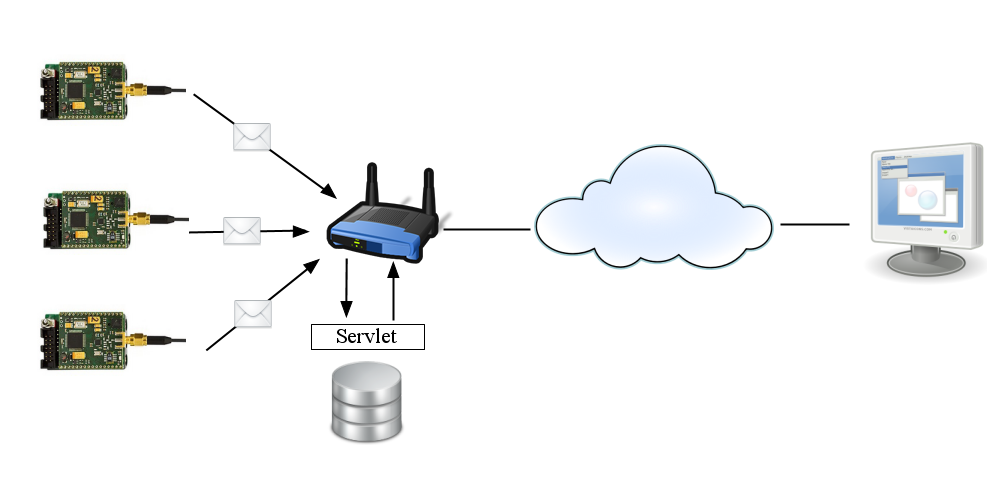
\includegraphics[width=12cm]{fig/Architektur.png}
   \caption{Architektur}
   \label{architecture}
\end{figure}


\section{Verwendetet Technologien} \labelSec{abschnitt}
\subsection{Linux Voyage \cite{voyage}} 
Als Betriebssystem für unseren Access Point haben wir uns für Voyage entschieden. Linux Voyage ist eine abgespeckte Version von Linux Debian, die für Access Points, Asterisk/VoIP Gateway und sonstigen Geräten geschrieben wurde. Da wir auf dem Access Point eine Flashkarte von 8 GB zur Verfügung hatten, war sich dieses Betriebssystem besonders gut geeignet, da es sehr  klein ist (128MB). Des weiteren sind alle wichtigen Treiber schon enthalten, welche wir für die WLAN Karte lediglich aktivieren mussten. \\
Ein weiterer Vorteil ist, dass weitere Software wie gewohnt über die Konsole installiert werden kann. So konnten wir recht einfach MySQL und Tomcat installieren.

\subsection{GWT \cite{gwt}}
Google Web Toolkit ist ein Toolkit zur Entwicklung und Optimierung von Browser-basierten Anwendungen \cite{gwt}. Der Code wird dabei vom Entwickler in Java geschrieben und anschließend vom GWT-Compiler in Javascript-Code umgewandelt. \\
Die Vorteile bei GWT sind:
\begin{itemize}
 \item Browser-Kompatibilität
 \item Testen in Java (Unit-Tests sind auch möglich)
 \item Entwickler benötigt keine Javascript Kenntnisse, da der Code in Java geschrieben wird
 \item viele Zusatz-Frameworks (z.B. Smart GWT)
 \item umfangreiche Dokumentation und Beispielanwendungen
\end{itemize}

Man muss allerdings erst den Aufbau von GWT verstehen, was am Anfang sehr aufwendig sein kann. So ist dieses Framework nicht unbedingt bei kleinen Anwendung zu empfehlen. \\
GWT war für unser Projekt sehr hilfreich, da die Webseite abhängig von dem Backend aufgebaut wurde und durch GWT-RPC eine einfache Anbindung an das Backend gegeben war.\\
\newline
Im Rahmen dieses Projektes wurde GWT als Plugin für Eclipse verwendet. Der Link für das Plugin ist der folgende: \cite{gwtplugin}.

\subsection{Smart GWT}
Smart GWT ist ein Framework, welches, basierend auf GWT, eine Vielzahl von Erweiterungen der Oberfläche anbietet. Da es viele Widgets anbietet, die GWT nicht besitzt, wurde es für dieses Projekt verwendet.\\
Dabei bietet Smart GWT über die Showcases (hier ein Link: \cite{smartgwt}) viele Codeschnipsel, die die Entwicklung  einfach gestalten. Des weiteren lässt sich Smart GWT sehr leicht in den Code einbinden. Der Nutzer lädt lediglich Jars herunter, die eingebunden werden müssen. \\
Der Nachteil von Smart GWT ist allerdings, dass man die Komponenten nicht mit Komponenten von GWT kombinieren sollte (also zum Beispiel sollte man keine Smart GWT Buttons in Layouts von GWT involvieren), da dies zu unerwarteten Effekten führen kann.\\
\newline
Möchte man Smart GWT nutzen, so muss die Jar-Datei (unter: \cite{smartgwtdown}) heruntergeladen werden und in den „Build Path“ eingebunden werden.\\
In der Datei „*.gwt.xml“ \footnote{steht f"ur den Namen des Web Application Projekts} muss nun noch die folgende Zeile eingefügt werden:

\lstset{language=HTML}
\begin{lstlisting}
<inherits name="com.smartgwt.SmartGwt"/>
\end{lstlisting}

\subsection{Charts von Google}
Google Visualization bietet viele Möglichkeiten, Charts und Tabellen in GWT zu erstellen. Dabei werden die Charts in Javascript geschrieben. Allerdings bietet Google auch ein Jar für GWT-Dateien an, so das an dieser Stelle der Programmierer Java-Code schreiben kann. \\
Um ein Chart zu erstellen, muss der Nutzer lediglich eine Datentabelle (DataTable) von Google erstellen und dabei die Formate der Eingabedaten festlegen. Diese Daten werden dem gewünschten Chart mitgegeben und dieser wird auf der Oberfläche dargestellt. Alles weitere wird mitgeliefert wie zum Beispiel die „Clickevents“, oder die dynamische Größenanpassung der Charts an die Menge der Daten.\\
Aber auch hier ist der Nachteil, dass man Charts von Google nicht einfach mit Smart GWT Elementen kombinieren kann, dafür aber mit GWT Elementen.\\
\newline
Um Google Charts nutzen zu können, muss man die Jar-Datei (unter: \cite{charts}) herunterladen und in das Projekt im „Build Path“ einbinden. In der Datei „*.gwt.xml“ muss nun die folgende Zeile eingefügt werden.
\lstset{language=HTML}
\begin{lstlisting}
<inherits name='com.google.gwt.visualization.Visualization'/>
\end{lstlisting}

\section{Sensor-Knoten}
Der verwendete Sensor-Knoten basiert auf dem MSB430H-Board. Es enthält mehrere Sensoren. Diese sind der SHT11-Sensor , welcher die Temperatur und Luftfeuchtigkeit misst und der MMA 7260Q G-Sensor, 
mit dem die relative Lage des Sensor-Knotens im Raum festgestellt werden kann. Der Sensor-Knoten wurde mit dem WLAN-Modul RN-134 der Firma Roving Networks über die UART-Schnittstelle fest verlötet. 
Die Kommunikation zwischen dem programmierbaren Board und dem WLAN-Modul erfolgt also über die serielle Schnittstelle. An dieser Schnittstelle wurde ein Kipp-Schalter und  ein serielles Kabel angebracht, 
welche es ermöglichen, den Daten-Austausch zwischen Board und Modul zu verfolgen. Damit fiel das Debuggen der Kommunikation leichter.

\subsection{HTTP-Kommunikation}
\label{ssec:HTTP}
Bei der Erprobung des WLAN-Moduls über eine serielle Schnittstelle haben wir verschiedene Übertragungsverfahren getestet: 

\begin{itemize}
 \item Das Modul bietet die Möglichkeit, alle x Sekunden einen UDP-Broadcast zu senden, welcher die auf dem Modul gesetzte Zeit beinhaltet und alle gemessenen Sensor-Werte. Dies ist für das Projekt nicht praktikabel, da die Sensoren nicht direkt an das WLAN-Modul angeschlossen sind, sondern an dem Sensor-Knoten. Deswegen ist auch der UDP-Unicast unbrauchbar.
 \item Das Modul bietet die Möglichkeit, eine TCP Auto-Connection zu nutzen, also automatisch alle x Sekunden aufzuwachen und eine TCP-Verbindung zu einem vordefinierten Host aufzurufen. Da das WLAN-Modul aber keine Werte vom Sensor-Knoten pollen kann, ist diese Methode ebenfalls unbrauchbar. 
 \item Eine weitere Methode, die aber ebenfalls wegen des oben beschriebenen Grundes fehlschlägt ist das automatische Senden von Sensor-Daten an einen HTTP-Server. 
\end{itemize}

Nach ausgiebigen Tests haben wir uns entschieden, die Daten über eine TCP-Verbindung zu verschicken. Diese wird von dem Sensor-Knoten geöffnet. Danach wird ein GET-Befehl des HTTP-Protokolls abgesetzt. Dabei wird angegeben, dass die Verbindung nicht geschlossen werden soll. Dies ermöglicht es (HTTP 1.1), mehrere Datensätze hintereinander mit Hilfe des GET-Befehls versendet, ohne die TCP-Verbindung jedes Mal neu initiieren zu müssen. Da die Verbindung nach ca. 5 Minuten vom Server geschlossen würde, muss sie in regelmäßigen Abständen vom Client geschlossen und direkt danach neu aufgebaut werden.  \\
Das WLAN-Modul verschickt einen festgelegten String (Default: „*HELLO* “), welcher nicht leer sein darf, beim erfolgreichen Aufbauen der TCP-Verbindung. Das hat uns zuerst Probleme bereitet hat, da der Tomcat-Server unbekannte Befehls-Präfices nicht ignoriert. Die Lösung ist das Benutzen von „GET“ als Communication-String. Da dieser aber nur beim Starten der Verbindung gesendet wird, muss jeder weitere GET-Befehl vollständig übertragen werden. Dies ist eine unschöne Lösung, allerdings lies sich das Problem nicht anders beheben, da das WLAN-Modul selbst nicht programmiert werden kann.

\subsection{Konfiguration des WLAN-Moduls}
Bei jedem Start des Sensor-Knotens muss das WLAN-Modul in einen wohldefinierten Zustand gebracht werden. Da beim Booten des Knotens nur schwer verifiziert werden kann, 
ob alle Einstellungen korrekt vorgenommen sind, haben wir uns dafür entschieden, dass das WLAN-Modul bei jedem Start auf die Fabrikeinstellungen  zurück gesetzt und dann neu konfiguriert wird. 
Dies ist nötig, da beim Programmieren der Sensor-Knoten zwar neu gestartet wurde beim Debuggen, die Stromversorgung des WLAN-Moduls aber nicht unterbrochen wurde und es so in einem beliebigen Zustand sein konnte. 
Das Zurücksetzen hat ebenfalls den Vorteil, dass das Modul nicht vor dem ersten Betrieb explizit initiiert werden muss, allerdings dauert jeder Boot-Vorgang etwas länger. Insgesamt jedoch werden bereits ca. 10 Sekunden nach dem Einschalten die ersten Sensor-Werte gesendet. 


\subsection{Programmierung des Sensor-Knotens}
Für die Programmierung des Sensor-Knotens wurde der Code Composer  [TODO: INSERT REAL NAME HERE] verwendet. Die Programmiersprache ist ein C-Dialekt, welcher fast alle Funktionen des Standards bereit stellt. \\
Das Programm des Sensor-Knotens besteht aus zwei Teilen: Zuerst wird eine Initalisierungs-Phase durchlaufen in der Interrupts angeschaltet werden, nötiger Speicher allociiert und das WLAN-Modul konfiguriert wird. Danach beginnt eine Endlos-Schleife, die das „Betriebssystem“ darstellt. 
In dieser Schleife werden die Sensor-Werte ermittelt und dann per WLAN verschickt.

\subsubsection{Initialisierung}
Bei der Initialisierung werden folgende Schritte chronologisch ausgeführt: 

\begin{itemize}
 \item Initialisierung der Port Register
 \item Aktivierung der quarzstabilen XT2 Taktquelle (7.3728MHz)
 \item Initialisierung der UART-RS232 Schnittstelle mit 9.6kBit/s
 \item Einschalten der Interrupts für die beiden Taster, Freigeben der Interrupts und  Aktivierung der Interrupt-Routinen
 \item Zurücksetzen des WLAN-Moduls in den Auslieferungszustand
 \item Setzen von WLAN-SSID, Passwort und anderen Parametern
 \item Verbindungsaufbau mit dem Access-Point und einrichten der TCP-Verbindung zum Tomcat-Server
\end{itemize}
Dann tritt das System in die zweite Phase ein.

\subsubsection{Betriebssystem}

Das „Betriebsystem“ besteht aus einer Endlos-Schleife, in der folgende Aktionen ausgeführt werden:
\begin{itemize}
 \item Überprüfung, ob bereits 20 Abfragen gesendet wurden; ggf. Trennung und erneuter Aufbau der TCP-Verbindung (der Server würde die Verbindung nach ca. 5 Minuten trennen)
 \item Auslesen der Sensoren, Aufbereitung der gelesenen Werte und Speicherung des Requests in einer Warteschlange, welche alle zu sendenden GET-Anfragen enthält
 \item Falls die Verbindung nicht gerade neu geöffnet wurde, wird „GET “ dem Request voran gestellt (Grund siehe Abschnitt \ref{ssec:HTTP})
 \item Solange noch weitere Requests in der Warteschlange sind, werden diese ebenfalls entfernt und dann versendet
\end{itemize}

\subsubsection{Tastendruck}
Die Erkennung eines Tastendrucks geschieht in dem in der Initialisierung definierten Interrupt. Dort wird direkt beim Interrupt und 0.5 Sekunden nach dem Auslösen gemessen, welcher Taster gedrückt wurde und dann beide Messungen logisch verodert. Damit können wir mit einem Interrupt ebenfalls feststellen, falls beide Taster gleichzeitig gedrückt wurden. Weiterhin kann damit ausgeschlossen werden, dass die analog gemessene Größe am Anfang noch etwas flackert und eventuell beim ersten Auslesen den falschen Wert liefert. Danach wird ein GET-Request für das Taster-Event erstellt und in die Warteschlange eingereiht. Beim nächsten Durchlauf der Betriebssystem-Schleife wird dieser Request dann ebenfalls mit verschickt. Die Auflösung der Tasten-Events ist damit gleich einem Schleifendurchlauf, der bei durchschnittlich 3 Sekunden, maximal bei 7 Sekunden (Trennen und neuer Aufbau der Verbindung) liegt. 

\section{Backend}\label{sec:backend}

\subsection{Daten-Verarbeitung}

\subsection{Daten-Bereitstellung}

\section{Frontend}
Die Sensoren, die im Haushalt verteilt sind, schicken die gemessenen Daten an den Access Point. Nun müssen diese Daten in geeigneter Weise aufbereitet werden und dem Nutzer zur Verfügung gestellt werden. Hierfür wurde eine Webseite gebaut, welche die gemessenen Daten in Diagrammen darstellen. \\
In diesem Kapitel wird dieses Frontend vorgestellt und beschrieben.

\subsection{Anforderungen}

An die Webseite, die es den Nutzer ermöglicht, die Daten der Sensoren zu überwachen, gibt es eine Reihe von Anforderungen. \\
Eine wichtige Anforderung ist die benutzerfreundliche Oberfläche, die in sich einfach gehalten ist und es den Anwender ermöglicht, sich schnell einzuarbeiten. Aus diesen Grund wurde die Oberfläche sehr schlicht gehalten und auf das Wesentliche reduziert.\\
Über eine Drop-down-Box kann der Nutzer zwischen den verschiedenen Sensoren auswählen und sich Daten anzeigen lassen. Dabei werden unterschiedliche Diagramme für die unterschiedlichen gemessenen Daten angezeigt. In unseren Fall hatten wir ein Diagramm für die Temperatur, Feuchtigkeit und 2 Diagramme für die Neigung des Sensors. Da es aber möglich sein soll, andere Sensoren an das System anzuschließen, welche andere Daten (Propertries) messen, passt sich die Oberfläche mit den Diagrammen an die jeweiligen Daten an.\\
Nun kann der Nutzer die gemessene Werte überwachen. Dabei hat dieser aber nur ein Diagramm gleichzeitig im Blick (da pro Diagramm ein Tab in einem Tab-Menü zur Verfügung steht). Es kann passieren, dass der Anwender so zum Beispiel nicht beobachten kann, dass die Temperatur im Kühlschrank stetig zunimmt, weil dieser das Diagramm mit der Neigung des Sensors geöffnet hat. Damit der Nutzer gewarnt wird, wurden Trigger in unser System integriert. Dabei wird in serverseitiger und clientseitiger Trigger unterschieden. Wird eine Aktion auf der Clientseite ausgelöst, so wird eine Dialogbox auf der Webseite angezeigt. Wird eine serverseitige Aktion ausgelöst, so wird eine System-Ausgabe auf der Konsole ausgegeben.\\
Eine weitere Anforderung an das System war es, dass der Standort eines Sensors bearbeitet werden kann und dieser dann in die Datenbank abgespeichert wird. Es kann passieren, dass der mobile Sensorknoten an einen anderen Ort platziert wird. Bei der Anzeige der Sensordaten kann der Benutzer auf „Edit“ klicken und den Ort des Sensors bearbeiten. Die ID und die IP sollen nicht geändert werden. \\
Alle diese Anforderungen sind für die leichte Bedienbarkeit der Oberfläche und wurde in diesem System umgesetzt.

\subsection{Projektaufbau}

Da für dieses Projekt GWT genutzt wurde, war der Aufbau des Frontends zum Teil durch die Struktur von GWT vorgegeben. \\
Unter dem Ordner „src/de/berlin/fu/client“ befindet sich die Datei „TelproGWT.java“ in der man Hauptteil des Frontends findet. In der Datei „TelproGWT.gwt.xml“, welche man in dem Verzeichnis „src/de/berlin/fu/berlin“ findet, wird definiert welche onModuleLoad-Methode welcher Klasse (in unserem Fall TeproGWT) aufgerufen werden soll. \\
Eine wichtiges Interface in diesem Projekt ist das Service-Interface„MyServer.java“, welche sich in dem Ordner „src/de/berlin/fu/shared“ findet. Diese gibt vor, welche Methoden von der Clientseite genutzt werden können und somit mit der Backendseite kommunizieren. Damit nun die Clientseite die Methoden der Serverseite nutzen kann, muss ein sogenanntes Async-Interface implementiert werden. Dieses befindet sich auch in dem Ordner „src/de/berlin/fu/shared“ und heißt „MyServerAsync.java“. Es wird ein asynchrones Interface definiert, da man vermeiden möchte, dass die Anwendung beim Aufruf der Methoden der Serverseite einfriert und der Anwender warten muss. Google Webtoolkit gibt diese Art von Interface beim GWT-RPC immer vor. In der Klasse, welche die Benutzeroberfläche implementiert, wird dieses Async-Interface initialisiert. 
In den anderen Packages befindet sich die Implementation der Backendseite, welche in dem Kapitel \ref{sec:backend} (Backend) näher erläutert wird.


\subsection{Code}
Die Klasse TelproGWT.java ist die Klasse, in der der Code der Clientseite steht. Jede Klasse in GWT, welche den Client-Code enthält, implementiert das Interface „EntryPoint“. Dabei wird von GWT vorgeschrieben, dass die Methode „onModuleLoad“ implementiert werden muss. Diese Methode wird aufrufen, sobald der Anwender die Webseite in dem Browser aufruft.\\
Wird die onModuleLoad-Methode aufgerufen, so holt sich die Clientseite als erstes alle Propertytypen und Eventtypen die in der Datenbank abgespeichert wurden. Diese Typen werden an mehreren Stelle im Code benötigt. Um nicht mehre Datenbankanfragen und somit die Anwendung langsamer zu machen, werden die Typen einmal abgefragt und in einer HashMap abgespeichert. \\
Mit den Propertytyen kann nun dynamisch die Ansicht für die Liniendiagramme aufgebaut werden. Pro Propertytyp wird ein Tab mit einem Liniendiagramm aufgebaut und in das Tab-Menü eingepflegt. Dieses Tab-Menü ermöglicht es, dass nur das Diagramm aktualisiert wird, welches gerade angezeigt wird. Da dieses alle 3 Sekunden aktualisiert wird, war dieser Schritt nötig, da dieses den Datenverkehr verringert und damit auch die Anwendung schneller macht.\\
Die Events werden in den 3 Sekunden immer mit aktualisiert und es ist egal, ob der Nutzer sich die Eventtabelle ansieht oder nicht. Löst ein Event nun eine Aktion aus (welche in dem Trigger definiert wurde), so soll der Anwender informiert werden (zum Beispiel über ein Dialogfenster), wenn dieser eintritt. So erhält man ein Warnsystem, welche wichtig für dieses System ist.\\
Durch GWT können nicht nur Oberflächenelemente eingefügt werden, sondern auch gestaltet werden. Zum Beispiel kann die Größe, Farbe, mit oder ohne Rahmen und vieles mehr eingestellt werden. Wie die Oberfläche aussieht, kann dem nächsten Kapitel und den darin enthaltenden Bildern entnommen werden.

\subsection{Screenshots}

Um einen Überblick über das Interface zu bekommen, sollen hier einige Screenshots gezeigt  werden.   

\begin{figure}[htbp]
   \centering
   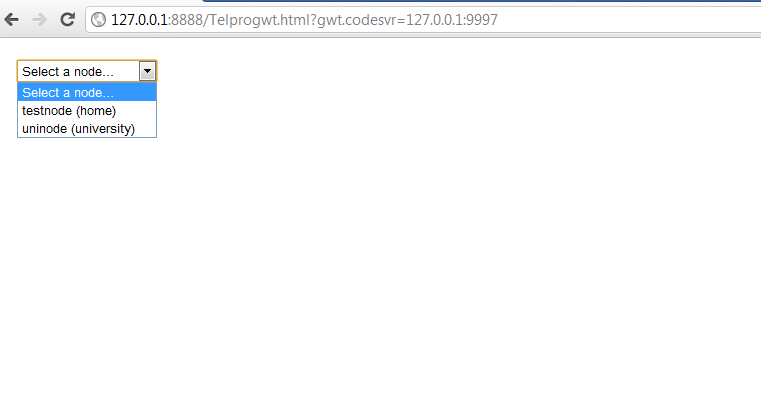
\includegraphics[width=12cm]{fig/screen1.png}
   \caption{Screenshot}
   \label{screen1}
\end{figure}

\begin{figure}[htbp]
   \centering
   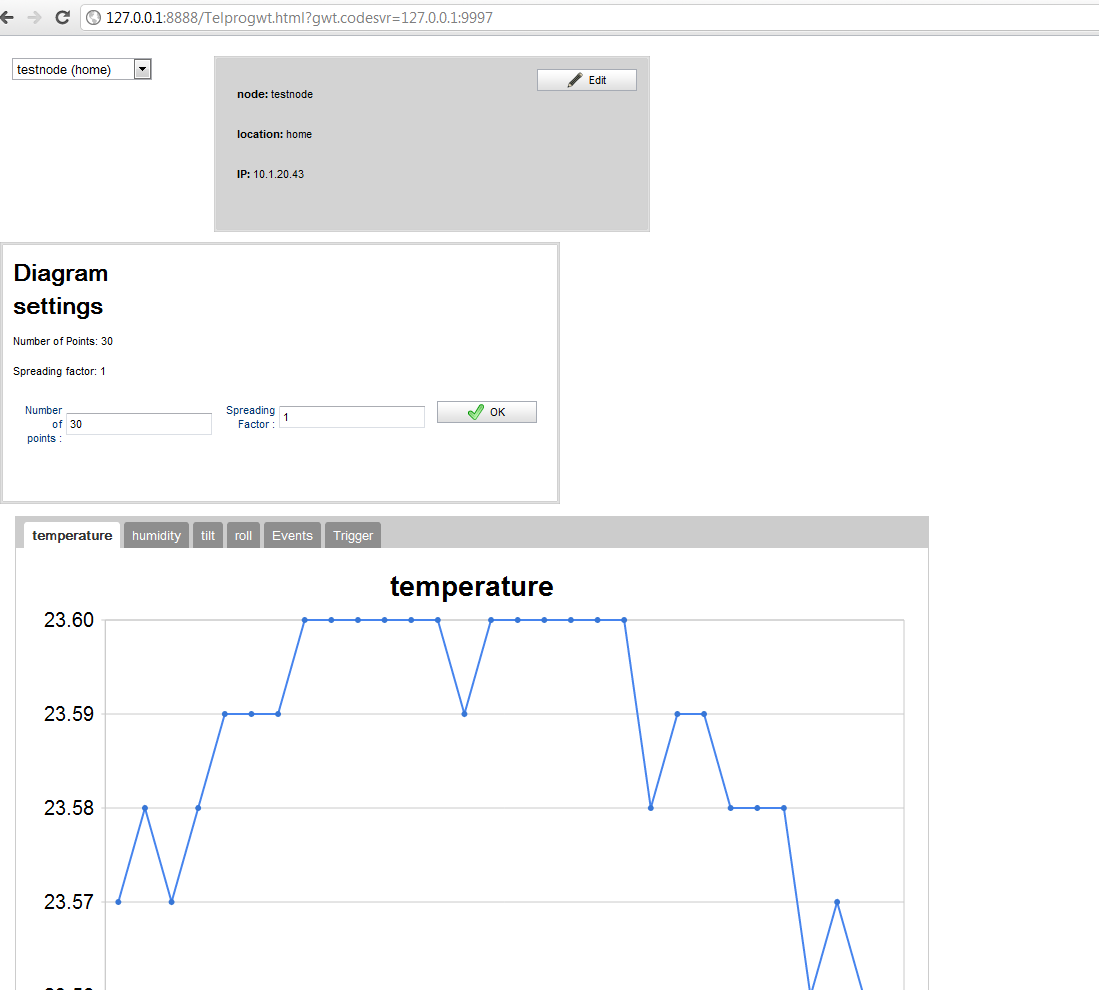
\includegraphics[width=12cm]{fig/screen2.png}
   \caption{Screenshot}
   \label{screen1}
\end{figure}

\begin{figure}[htbp]
   \centering
   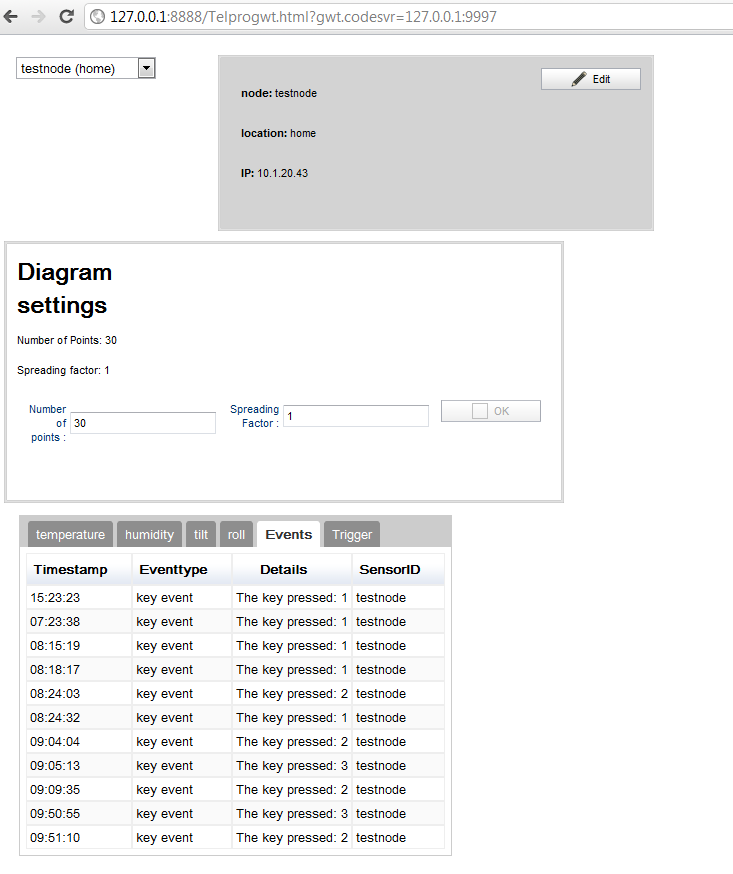
\includegraphics[width=12cm]{fig/screen3.png}
   \caption{Screenshot}
   \label{screen1}
\end{figure}

\begin{figure}[htbp]
   \centering
   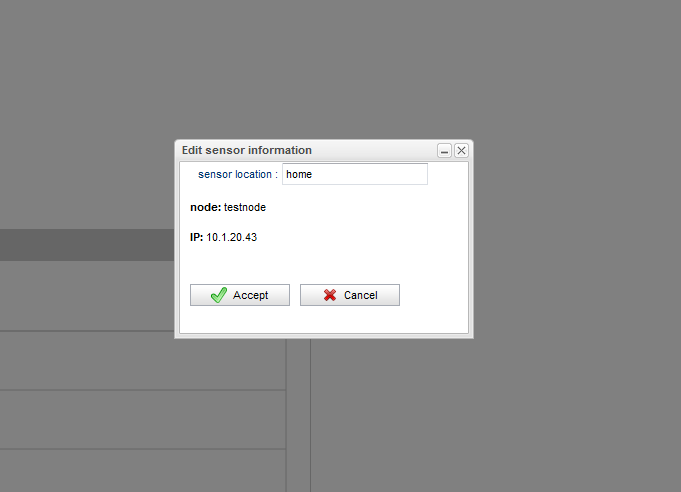
\includegraphics[width=12cm]{fig/screen4.png}
   \caption{Screenshot}
   \label{screen1}
\end{figure}
  
\section{Ausblick} \labelSec{ausblick}

\clearpage

\section{Appendix}

% @SETTINGS: Insert the name of your bibliography file WITHOUT extension.
\bibliography{main}

\bibliographystyle{abbrv}

\end{document}
